% Options for packages loaded elsewhere
\PassOptionsToPackage{unicode}{hyperref}
\PassOptionsToPackage{hyphens}{url}
%
\documentclass[
]{book}
\title{Portfólio Gabriel Maciel}
\author{Gabriel Maciel}
\date{2022-05-25}

\usepackage{amsmath,amssymb}
\usepackage{lmodern}
\usepackage{iftex}
\ifPDFTeX
  \usepackage[T1]{fontenc}
  \usepackage[utf8]{inputenc}
  \usepackage{textcomp} % provide euro and other symbols
\else % if luatex or xetex
  \usepackage{unicode-math}
  \defaultfontfeatures{Scale=MatchLowercase}
  \defaultfontfeatures[\rmfamily]{Ligatures=TeX,Scale=1}
\fi
% Use upquote if available, for straight quotes in verbatim environments
\IfFileExists{upquote.sty}{\usepackage{upquote}}{}
\IfFileExists{microtype.sty}{% use microtype if available
  \usepackage[]{microtype}
  \UseMicrotypeSet[protrusion]{basicmath} % disable protrusion for tt fonts
}{}
\makeatletter
\@ifundefined{KOMAClassName}{% if non-KOMA class
  \IfFileExists{parskip.sty}{%
    \usepackage{parskip}
  }{% else
    \setlength{\parindent}{0pt}
    \setlength{\parskip}{6pt plus 2pt minus 1pt}}
}{% if KOMA class
  \KOMAoptions{parskip=half}}
\makeatother
\usepackage{xcolor}
\IfFileExists{xurl.sty}{\usepackage{xurl}}{} % add URL line breaks if available
\IfFileExists{bookmark.sty}{\usepackage{bookmark}}{\usepackage{hyperref}}
\hypersetup{
  pdftitle={Portfólio Gabriel Maciel},
  pdfauthor={Gabriel Maciel},
  hidelinks,
  pdfcreator={LaTeX via pandoc}}
\urlstyle{same} % disable monospaced font for URLs
\usepackage{color}
\usepackage{fancyvrb}
\newcommand{\VerbBar}{|}
\newcommand{\VERB}{\Verb[commandchars=\\\{\}]}
\DefineVerbatimEnvironment{Highlighting}{Verbatim}{commandchars=\\\{\}}
% Add ',fontsize=\small' for more characters per line
\usepackage{framed}
\definecolor{shadecolor}{RGB}{248,248,248}
\newenvironment{Shaded}{\begin{snugshade}}{\end{snugshade}}
\newcommand{\AlertTok}[1]{\textcolor[rgb]{0.94,0.16,0.16}{#1}}
\newcommand{\AnnotationTok}[1]{\textcolor[rgb]{0.56,0.35,0.01}{\textbf{\textit{#1}}}}
\newcommand{\AttributeTok}[1]{\textcolor[rgb]{0.77,0.63,0.00}{#1}}
\newcommand{\BaseNTok}[1]{\textcolor[rgb]{0.00,0.00,0.81}{#1}}
\newcommand{\BuiltInTok}[1]{#1}
\newcommand{\CharTok}[1]{\textcolor[rgb]{0.31,0.60,0.02}{#1}}
\newcommand{\CommentTok}[1]{\textcolor[rgb]{0.56,0.35,0.01}{\textit{#1}}}
\newcommand{\CommentVarTok}[1]{\textcolor[rgb]{0.56,0.35,0.01}{\textbf{\textit{#1}}}}
\newcommand{\ConstantTok}[1]{\textcolor[rgb]{0.00,0.00,0.00}{#1}}
\newcommand{\ControlFlowTok}[1]{\textcolor[rgb]{0.13,0.29,0.53}{\textbf{#1}}}
\newcommand{\DataTypeTok}[1]{\textcolor[rgb]{0.13,0.29,0.53}{#1}}
\newcommand{\DecValTok}[1]{\textcolor[rgb]{0.00,0.00,0.81}{#1}}
\newcommand{\DocumentationTok}[1]{\textcolor[rgb]{0.56,0.35,0.01}{\textbf{\textit{#1}}}}
\newcommand{\ErrorTok}[1]{\textcolor[rgb]{0.64,0.00,0.00}{\textbf{#1}}}
\newcommand{\ExtensionTok}[1]{#1}
\newcommand{\FloatTok}[1]{\textcolor[rgb]{0.00,0.00,0.81}{#1}}
\newcommand{\FunctionTok}[1]{\textcolor[rgb]{0.00,0.00,0.00}{#1}}
\newcommand{\ImportTok}[1]{#1}
\newcommand{\InformationTok}[1]{\textcolor[rgb]{0.56,0.35,0.01}{\textbf{\textit{#1}}}}
\newcommand{\KeywordTok}[1]{\textcolor[rgb]{0.13,0.29,0.53}{\textbf{#1}}}
\newcommand{\NormalTok}[1]{#1}
\newcommand{\OperatorTok}[1]{\textcolor[rgb]{0.81,0.36,0.00}{\textbf{#1}}}
\newcommand{\OtherTok}[1]{\textcolor[rgb]{0.56,0.35,0.01}{#1}}
\newcommand{\PreprocessorTok}[1]{\textcolor[rgb]{0.56,0.35,0.01}{\textit{#1}}}
\newcommand{\RegionMarkerTok}[1]{#1}
\newcommand{\SpecialCharTok}[1]{\textcolor[rgb]{0.00,0.00,0.00}{#1}}
\newcommand{\SpecialStringTok}[1]{\textcolor[rgb]{0.31,0.60,0.02}{#1}}
\newcommand{\StringTok}[1]{\textcolor[rgb]{0.31,0.60,0.02}{#1}}
\newcommand{\VariableTok}[1]{\textcolor[rgb]{0.00,0.00,0.00}{#1}}
\newcommand{\VerbatimStringTok}[1]{\textcolor[rgb]{0.31,0.60,0.02}{#1}}
\newcommand{\WarningTok}[1]{\textcolor[rgb]{0.56,0.35,0.01}{\textbf{\textit{#1}}}}
\usepackage{longtable,booktabs,array}
\usepackage{calc} % for calculating minipage widths
% Correct order of tables after \paragraph or \subparagraph
\usepackage{etoolbox}
\makeatletter
\patchcmd\longtable{\par}{\if@noskipsec\mbox{}\fi\par}{}{}
\makeatother
% Allow footnotes in longtable head/foot
\IfFileExists{footnotehyper.sty}{\usepackage{footnotehyper}}{\usepackage{footnote}}
\makesavenoteenv{longtable}
\usepackage{graphicx}
\makeatletter
\def\maxwidth{\ifdim\Gin@nat@width>\linewidth\linewidth\else\Gin@nat@width\fi}
\def\maxheight{\ifdim\Gin@nat@height>\textheight\textheight\else\Gin@nat@height\fi}
\makeatother
% Scale images if necessary, so that they will not overflow the page
% margins by default, and it is still possible to overwrite the defaults
% using explicit options in \includegraphics[width, height, ...]{}
\setkeys{Gin}{width=\maxwidth,height=\maxheight,keepaspectratio}
% Set default figure placement to htbp
\makeatletter
\def\fps@figure{htbp}
\makeatother
\setlength{\emergencystretch}{3em} % prevent overfull lines
\providecommand{\tightlist}{%
  \setlength{\itemsep}{0pt}\setlength{\parskip}{0pt}}
\setcounter{secnumdepth}{5}
\usepackage{booktabs}
\ifLuaTeX
  \usepackage{selnolig}  % disable illegal ligatures
\fi
\usepackage[]{natbib}
\bibliographystyle{plainnat}

\begin{document}
\maketitle

{
\setcounter{tocdepth}{1}
\tableofcontents
}
\hypertarget{sobre-mim}{%
\chapter{Sobre Mim}\label{sobre-mim}}


\includegraphics[width=3.125in,height=\textheight]{C:/Users/gabri/Documents/Projetos/Portfolio/Gabriel Maciel.jpeg}

Olá, bem vindo ao meu portfólio de ciência de dados, nele eu vou falar um pouco sobre minha relação com estatística e ciência de dados, mostrar minhas habilidades e experiências profissionais.

E-mail: \href{mailto:gabrielmacieldias@hotmail.com}{\nolinkurl{gabrielmacieldias@hotmail.com}}

Celular: (31) 98905-9541

\hypertarget{quem-sou-eu}{%
\section{Quem sou eu?}\label{quem-sou-eu}}

Meu nome é Gabriel Maciel Dias, tenho 23 anos e moro na cidade de Belo Horizonte.

Ingressei no curso de Estatística na UFMG em 2017 através do Enem, onde tive o primeiro contato com o mundo dos dados, desde então venho aprendendo sobre ciência de dados e como ela pode resolver problemas de diversas áreas.

Durante minha trajetória na graduação passei por estágios em diferentes áreas, comecei com uma rápida passagem no Hospital Odilon Behrens, no qual fazia análises voltada para saúde, m seguida fiz a transição para a própria UFMG, trabalhando como estagiário na Prograd fazendo grandes relatórios internos e públicos para avaliar qual é performace dos dicentes da UFMG, bem como o perfil dos ingressantes pelo SiSU.

Depois desses estágios comecei minha carreira na área de crédito, iniciei no Banco BDMG onde vi os primeiros modelos de risco, modelagem de perda e estudos de fraude voltados para pessoa jurídica. Trabalhei também no Banco BS2, vendo novamentes os modelos de crédito para pessoa jurídica e também para pessoa física, lá tive mais contato com os desenvolvedores que criavam as API´s e engenheiros de dados que preparavam os bancos de dados para as análises.

Atualmente trabalho como Assistente de Crédito no Banco Semear, no qual posso ter ainda mais contato com as esteiras e modelos de créditos, aprendendo diariamente sobre a parte operacional e teórica do crédito.

\hypertarget{formauxe7uxe3o}{%
\section{Formação}\label{formauxe7uxe3o}}

Bacharel em Estatística na Universidade Federal de Minas Gerais (UFMG) 2017 - 2021

\hypertarget{experiuxeancia-profissional}{%
\section{Experiência Profissional}\label{experiuxeancia-profissional}}

Desde que comecei na graduação passei por alguns estágios em áreas diferentes. Atualmente trabalho como Assistente de Crédito no Banco Semear e também como cientista de dados na Startup Sua Rua.

\hypertarget{hospital-odilon-behrens}{%
\subsection{Hospital Odilon Behrens}\label{hospital-odilon-behrens}}

Cargo: Estagiário de Estatística - Abril/2018 à Outubro/2018

Responsável pela confecção de relatórios mensais, além do atendimento de demanda de dados, fazendo a retirada deles em um banco específico do hospital. Durante esse período de trabalho elaborei alguns códigos na linguagem de programação R com o objetivo de aperfeiçoar relatórios e análises de dados.

\hypertarget{prograd-ufmg}{%
\subsection{Prograd UFMG}\label{prograd-ufmg}}

Cargo: Estagiário no Setor de Estatística da Prograd UFMG - Novembro/2018 à Junho/2020

Responsável pela elaboração de relatórios com análises descritivas e modelos de regressão, com finalidade de analisar o perfil e o desempenho dos estudantes da UFMG e divulgar o resultado em sites da universidade. Além disso, eram atendidos demandas de dados feitas por funcionários da universidade. Neste período os relatórios foram feitos usando o software R em conjunto com o R Markdown, Latex e excel.

\hypertarget{banco-de-desenvolvimento-de-minas-gerais---bdmg}{%
\subsection{Banco de Desenvolvimento de Minas Gerais - BDMG}\label{banco-de-desenvolvimento-de-minas-gerais---bdmg}}

Cargo: Estagiário de Crédito -- Julho/2020 à Dezembro/2020

Responsável pela conferência de planilhas de classificação de risco e criação de programa em R para automatizar determinadas conferências de dados. Além disso, também faço trabalhos com simulações (em Python e R) de carteiras de crédito para prever possíveis perdas. Fiz a criação de um programa em R que fazia a leitura e interpretação de PDF´s que verificavam possíveis anomalias, além disso, trabalhei diretamente com análise de fraude.

\hypertarget{banco-bs2}{%
\subsection{Banco BS2}\label{banco-bs2}}

Cargo: Estagiário de Crédito -- Janeiro/2021 à Agosto/2021

Responsável pelos atendimentos de ordens de serviço relacionado a dúvidas sobre análise de crédito além verificar como está o andamento de uma solicitação de crédito dentro do sistema do banco. Além disso, também trabalho na confecção de relatórios Backtest em R em conjunto com R Markdown com base de dados retiradas do SQL Server para verificar como a esteira de crédito está funcionando e se ela está tomando boas decisões de previsão.

\hypertarget{banco-semear}{%
\subsection{Banco Semear}\label{banco-semear}}

Cargo: Assistente de Crédito - Setembro/2021 - Atualmente

Responsável por criação de dashboards para tomada de decisões usando dados de carteira e esteira de crédito. Participo de comitês de crédito, reuniões com fornecedores de dados e de modelos e reuniões com lojistas do banco.
Faço também rateio e pagamento de fornecedores, estudo de base de dados para pré aprovado, bem como sugestões de análises que podem ajudar na resolução de problemas de negócio.
Todas as análises faço através do software R em conjunto com o Shiny e Excel.

\hypertarget{sua-rua}{%
\subsection{Sua Rua}\label{sua-rua}}

Cargo: Cientista de Dados - Agosto/2021 - Atualmente

Nessa startup trabalho com construção de modelos de dados geográficos, trabalhando com R e QGis, além disso atuo coletando dados e criando robôs para fazer Web Scrapping.

\hypertarget{habilidades}{%
\section{Habilidades}\label{habilidades}}

Programação avançada em R

Criação de relatórios com R Markdown

Criação de Dashboards com Shiny

Inglês intermediário

Pacote Office

\hypertarget{projetos}{%
\chapter{Projetos}\label{projetos}}

Abaixo tenho alguns projetos análises de dados que fiz para treinar algumas habilidades.

\hypertarget{banco-iris}{%
\section{Banco Iris}\label{banco-iris}}

Para primeira análise não tinha como ser diferente, vou começar com o dataset Iris, que é uma das bases de dados mais utilizadas para fazer análises básicas.

Para verificar a estrutura do banco de dados iris podemos usar a função ``head'':

\begin{Shaded}
\begin{Highlighting}[]
\FunctionTok{head}\NormalTok{(iris)}
\end{Highlighting}
\end{Shaded}

\begin{verbatim}
##   Sepal.Length Sepal.Width Petal.Length Petal.Width Species
## 1          5.1         3.5          1.4         0.2  setosa
## 2          4.9         3.0          1.4         0.2  setosa
## 3          4.7         3.2          1.3         0.2  setosa
## 4          4.6         3.1          1.5         0.2  setosa
## 5          5.0         3.6          1.4         0.2  setosa
## 6          5.4         3.9          1.7         0.4  setosa
\end{verbatim}

Usando a função ``head'' podemos ver as primeiras linhas da base de dados e suas colunas.

Segundo o \href{https://archive.ics.uci.edu/ml/datasets/iris}{UCI Machine Learning}, a base do Iris contém ao todo 150 linhas com 5 colunas, sendo:

\begin{itemize}
\tightlist
\item
  Sepal.Length = comprimento das sépalas (em cm);
\item
  Sepal.Width = largura das sépalas (em cm);
\item
  Petal.Lengt = comprimento das pétalas (em cm);
\item
  Petal.Width = largura das pétalas (em cm);
\item
  Species = espécie das plantas;
\end{itemize}

Para saber com qual análise posso começar vou verificar antes as classes das variáveis usando a função ``glimpse'' do pacote ``dplyr''.

\begin{Shaded}
\begin{Highlighting}[]
\CommentTok{\# Carregando a função dplyr}

\FunctionTok{library}\NormalTok{(dplyr)}
\end{Highlighting}
\end{Shaded}

\begin{verbatim}
## Warning: package 'dplyr' was built under R version 4.1.3
\end{verbatim}

\begin{Shaded}
\begin{Highlighting}[]
\FunctionTok{glimpse}\NormalTok{(iris)}
\end{Highlighting}
\end{Shaded}

\begin{verbatim}
## Rows: 150
## Columns: 5
## $ Sepal.Length <dbl> 5.1, 4.9, 4.7, 4.6, 5.0, 5.4, 4.6, 5.0, 4.4, 4.9, 5.4, 4.~
## $ Sepal.Width  <dbl> 3.5, 3.0, 3.2, 3.1, 3.6, 3.9, 3.4, 3.4, 2.9, 3.1, 3.7, 3.~
## $ Petal.Length <dbl> 1.4, 1.4, 1.3, 1.5, 1.4, 1.7, 1.4, 1.5, 1.4, 1.5, 1.5, 1.~
## $ Petal.Width  <dbl> 0.2, 0.2, 0.2, 0.2, 0.2, 0.4, 0.3, 0.2, 0.2, 0.1, 0.2, 0.~
## $ Species      <fct> setosa, setosa, setosa, setosa, setosa, setosa, setosa, s~
\end{verbatim}

Sabendo que as classes são númericas vou utilizar o ``summary'' para uma visão geral.

\begin{Shaded}
\begin{Highlighting}[]
\FunctionTok{summary}\NormalTok{(iris[,}\DecValTok{1}\SpecialCharTok{:}\DecValTok{4}\NormalTok{])}
\end{Highlighting}
\end{Shaded}

\begin{verbatim}
##   Sepal.Length    Sepal.Width     Petal.Length    Petal.Width   
##  Min.   :4.300   Min.   :2.000   Min.   :1.000   Min.   :0.100  
##  1st Qu.:5.100   1st Qu.:2.800   1st Qu.:1.600   1st Qu.:0.300  
##  Median :5.800   Median :3.000   Median :4.350   Median :1.300  
##  Mean   :5.843   Mean   :3.057   Mean   :3.758   Mean   :1.199  
##  3rd Qu.:6.400   3rd Qu.:3.300   3rd Qu.:5.100   3rd Qu.:1.800  
##  Max.   :7.900   Max.   :4.400   Max.   :6.900   Max.   :2.500
\end{verbatim}

Ao analisar os resultados pode-se notar que o comprimento das sépalas e pétalas é maior do que a largura dos mesmos.

Após observar brevemente o banco Iris gostaria de responder as seguintes perguntas:

\begin{itemize}
\tightlist
\item
  O tamanho de sépala e as espécies influenciam no tamanho de pétala?
\item
  Se sim, qual é essa relação?
\end{itemize}

\hypertarget{anuxe1lise-descritiva}{%
\subsection{Análise descritiva}\label{anuxe1lise-descritiva}}

Para responder essa pergunta vou começar com análise descritivas, que podem ser simples mas que em muitos casos já conseguem identificar informações valiosas

Vou partir do pressuposto que a média entre comprimento e largura de sépalas e pétalas é um bom indicador do seu tamanho, então farei isso no R.

\begin{Shaded}
\begin{Highlighting}[]
\NormalTok{iris }\OtherTok{\textless{}{-}}\NormalTok{ iris }\SpecialCharTok{\%\textgreater{}\%}
  \FunctionTok{mutate}\NormalTok{(}\AttributeTok{media\_petala =}\NormalTok{ (Petal.Length}\SpecialCharTok{+}\NormalTok{Petal.Width)}\SpecialCharTok{/}\DecValTok{2}\NormalTok{, }\CommentTok{\# Média das pétalas}
         \AttributeTok{media\_sepala =}\NormalTok{ (Sepal.Length}\SpecialCharTok{+}\NormalTok{Sepal.Width)}\SpecialCharTok{/}\DecValTok{2}\NormalTok{) }\SpecialCharTok{\%\textgreater{}\%} \CommentTok{\# Média das sépalas}
  \FunctionTok{select}\NormalTok{(media\_petala,media\_sepala,Species)}

\FunctionTok{head}\NormalTok{(iris, }\DecValTok{5}\NormalTok{)}
\end{Highlighting}
\end{Shaded}

\begin{verbatim}
##   media_petala media_sepala Species
## 1         0.80         4.30  setosa
## 2         0.80         3.95  setosa
## 3         0.75         3.95  setosa
## 4         0.85         3.85  setosa
## 5         0.80         4.30  setosa
\end{verbatim}

Podemos ver acima como ficou o banco de dados agora com apenas 3 variáveis.

Primeiramente farei um gráfico para verificar visualmente se há uma possível relação entre a média de comprimento e largura das pétalas e sépalas.

\begin{Shaded}
\begin{Highlighting}[]
\CommentTok{\# Carregando a função do ggplot2}

\FunctionTok{library}\NormalTok{(ggplot2)}

\FunctionTok{ggplot}\NormalTok{(iris) }\SpecialCharTok{+}
  \FunctionTok{geom\_point}\NormalTok{(}\FunctionTok{aes}\NormalTok{(}\AttributeTok{x =}\NormalTok{ media\_sepala,}\AttributeTok{y =}\NormalTok{ media\_petala)) }\SpecialCharTok{+}
  \FunctionTok{labs}\NormalTok{(}\AttributeTok{title =} \StringTok{"Relação Pétalas e Sépalas"}\NormalTok{,}
       \AttributeTok{x =} \StringTok{"Média Sépalas"}\NormalTok{,}
       \AttributeTok{y =} \StringTok{"Média Pétalas"}\NormalTok{) }\SpecialCharTok{+}
  \FunctionTok{theme\_bw}\NormalTok{()}
\end{Highlighting}
\end{Shaded}

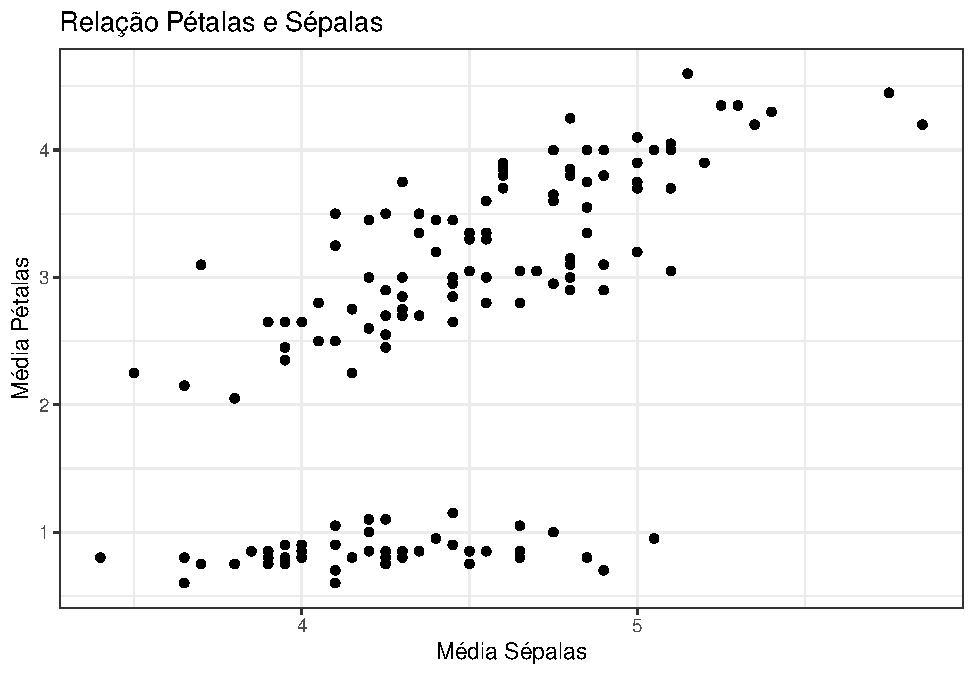
\includegraphics{_main_files/figure-latex/unnamed-chunk-5-1.pdf}

É possível notar que parece existir alguma relação, porém o efeito das espécies não nos permite enxergar isso da melhor forma, então vou segmentar o gráfico de acordo com a espécie.

\begin{Shaded}
\begin{Highlighting}[]
\FunctionTok{ggplot}\NormalTok{(iris) }\SpecialCharTok{+}
  \FunctionTok{geom\_point}\NormalTok{(}\FunctionTok{aes}\NormalTok{(}\AttributeTok{x =}\NormalTok{ media\_sepala,}\AttributeTok{y =}\NormalTok{ media\_petala)) }\SpecialCharTok{+}
  \FunctionTok{labs}\NormalTok{(}\AttributeTok{title =} \StringTok{"Relação Pétalas e Sépalas"}\NormalTok{,}
       \AttributeTok{x =} \StringTok{"Média Sépalas"}\NormalTok{,}
       \AttributeTok{y =} \StringTok{"Média Pétalas"}\NormalTok{) }\SpecialCharTok{+}
  \FunctionTok{theme\_bw}\NormalTok{() }\SpecialCharTok{+}
  \FunctionTok{facet\_grid}\NormalTok{(}\SpecialCharTok{\textasciitilde{}}\NormalTok{ Species)}
\end{Highlighting}
\end{Shaded}

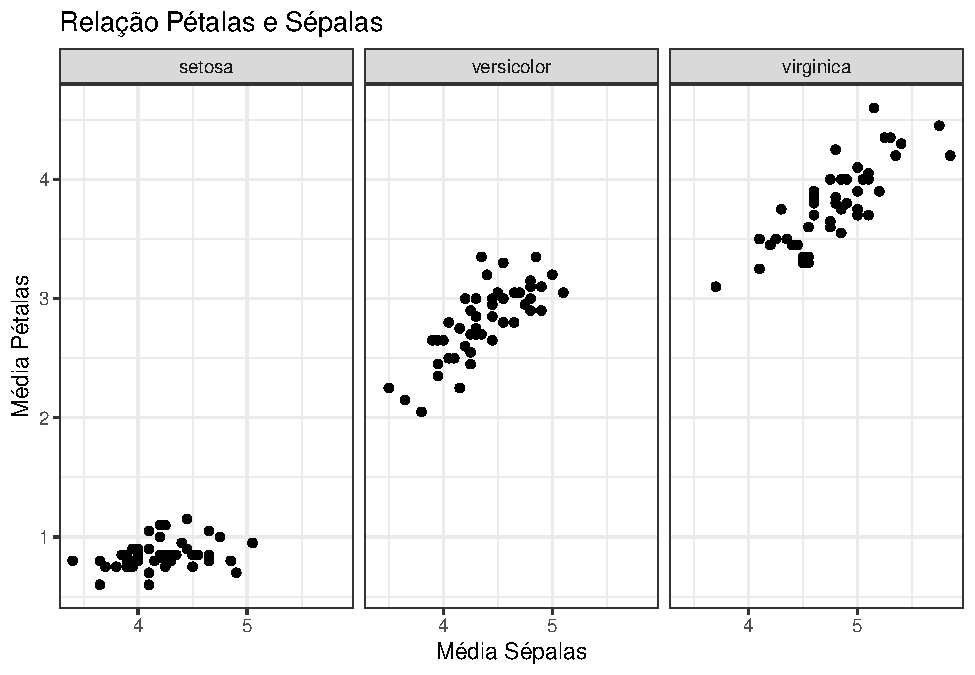
\includegraphics{_main_files/figure-latex/unnamed-chunk-6-1.pdf}

Agora podemos notar que as espécies parecem influenciar no tamanho das pétalas e sépalas, visto que os pontos se encontram em locais distintos dos gráficos. Além disso, nota-se possível relação positiva entre tamanho de sépalas e pétalas nas espécies versicolor e virginica, já a setosa não apresenta graficamente essa relação.

\hypertarget{anuxe1lise-de-regressuxe3o}{%
\subsection{Análise de Regressão}\label{anuxe1lise-de-regressuxe3o}}

Para avaliar se realmente existe essa relação estatística entre as pétalas, sépalas e espécie de planta eu vou usar a técnica de regressão linear.

\begin{Shaded}
\begin{Highlighting}[]
\CommentTok{\# Usando a função lm para ajustar o modelo}

\NormalTok{fit }\OtherTok{\textless{}{-}} \FunctionTok{lm}\NormalTok{(media\_petala}\SpecialCharTok{\textasciitilde{}}\NormalTok{media\_sepala}\SpecialCharTok{+}\NormalTok{Species, }\AttributeTok{data =}\NormalTok{ iris)}

\CommentTok{\# Usando a função summary para avaliar resultados dos ajustes}

\FunctionTok{summary}\NormalTok{(fit)}
\end{Highlighting}
\end{Shaded}

\begin{verbatim}
## 
## Call:
## lm(formula = media_petala ~ media_sepala + Species, data = iris)
## 
## Residuals:
##      Min       1Q   Median       3Q      Max 
## -0.50872 -0.13092  0.00096  0.14311  0.61936 
## 
## Coefficients:
##                   Estimate Std. Error t value Pr(>|t|)    
## (Intercept)       -1.33611    0.18761  -7.122 4.49e-11 ***
## media_sepala       0.51935    0.04398  11.809  < 2e-16 ***
## Speciesversicolor  1.86837    0.04055  46.073  < 2e-16 ***
## Speciesvirginica   2.64209    0.04716  56.025  < 2e-16 ***
## ---
## Signif. codes:  0 '***' 0.001 '**' 0.01 '*' 0.05 '.' 0.1 ' ' 1
## 
## Residual standard error: 0.2005 on 146 degrees of freedom
## Multiple R-squared:  0.9749, Adjusted R-squared:  0.9744 
## F-statistic:  1893 on 3 and 146 DF,  p-value: < 2.2e-16
\end{verbatim}

Acima temos alguns resultados interessantes, primeiramente é possível notar que o tamanho médio das sépalas e a espécie influencia no tamanho médio das pétalas, chego nessa conclusão pois o p-valor do modelos para cada um das variáveis é menor que 0,05.

A cada unidade que aumentamos no tamanho médio das sépalas, 0,51 é adicionado no tamanho médio das pétalas. Já quanto as espécies, o tamanho das pétalas na espécie Versicolor é 1,86 vezes maior que na espécie Setosa (que está oculto nos resultados) enquanto as pétalas na espécie Virginica são 2,64 vezes maiores que na Setosa.

Além disso, o R² foi de 0,9744, isso indica que aproximadamente 97\% da variação do tamanho das pétalas é explicada pelo tamanho das sépalas e espécie.

Antes de chegar a uma conclusão final dos resultados devemos verificar algumas suposições. Para o modelo de regressão linear é necessário normalidade e homocedasticidade dos resíduos.

\begin{Shaded}
\begin{Highlighting}[]
\CommentTok{\# Teste de normalidade de Shapiro Wilk}

\FunctionTok{shapiro.test}\NormalTok{(fit}\SpecialCharTok{$}\NormalTok{residuals)}
\end{Highlighting}
\end{Shaded}

\begin{verbatim}
## 
##  Shapiro-Wilk normality test
## 
## data:  fit$residuals
## W = 0.99395, p-value = 0.7868
\end{verbatim}

O p-valor do teste de Shapiro Wilk foi de 0,7868, dessa forma concluímos que os resíduos seguem a distribuição normal.

\begin{Shaded}
\begin{Highlighting}[]
\CommentTok{\# Verificação de homocedasticidade}

\FunctionTok{plot}\NormalTok{(fit}\SpecialCharTok{$}\NormalTok{fitted.values,fit}\SpecialCharTok{$}\NormalTok{residuals)}
\end{Highlighting}
\end{Shaded}

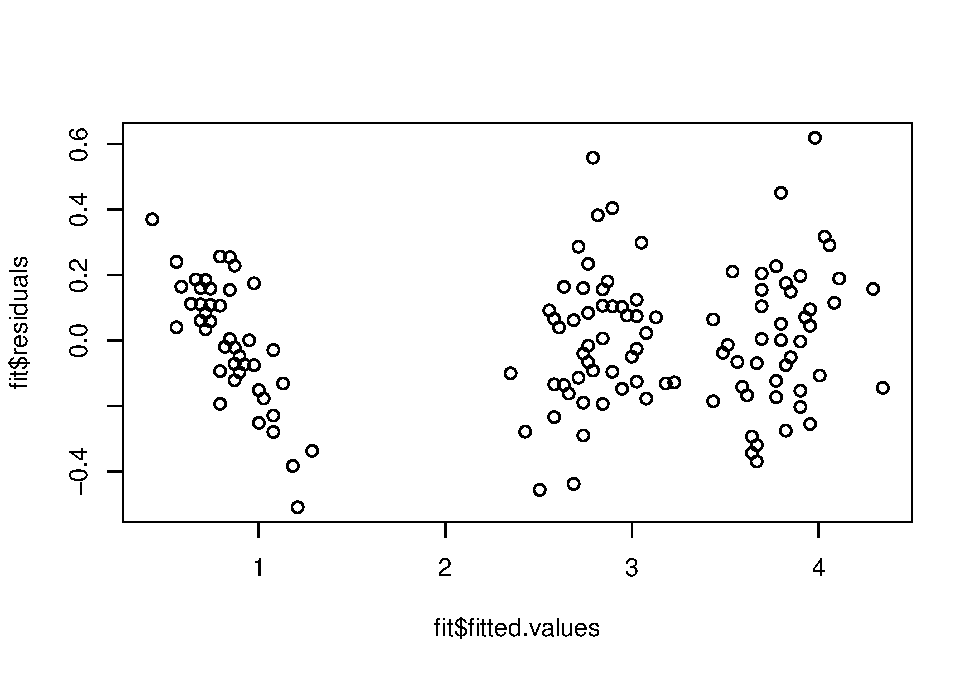
\includegraphics{_main_files/figure-latex/unnamed-chunk-9-1.pdf}

Acima temos o gráfico dos resíduos pelo valores ajustados, a dispersão dos resíduos ao longo do eixo dos valores ajustados parece ser a mesma, esse é um grande indicativo de homocedasticidade dos resíduos, ou seja, variância constante.

\hypertarget{conclusuxe3o}{%
\subsection{Conclusão}\label{conclusuxe3o}}

Com os pressupostos verificados posso chegar a uma conclusão respondendo as perguntas feitas no início.

O tamanho de sépala e tipo de espécie influenciam sim no tamanho das pétalas, e essa relação acontece da seguinte forma:

\begin{itemize}
\tightlist
\item
  O tamanho de sépala tem uma relação positiva com o tamanho das pétalas, ou seja, quanto maior são as sépalas, maiores vão ser as pétalas.
\item
  As espécies Virginica e Versicolor apresentam tamanho de pétala maior em relação a espécie Setosa
\end{itemize}

\hypertarget{data-sciente-e-credit-scoring}{%
\section{Data Sciente e credit scoring}\label{data-sciente-e-credit-scoring}}

Como grande entusiasta de modelos estatísticos e de crédito, busco sempre reter mais conhecimento sobre isso, nas últimas semanas venho lendo o livro Credit Scoring do Abharam Laredo. Nele o autor passa toda sua experiência sobre esse tema e no final fornece alguns bancos de dados e um ``problema'' que pode ser utilizado para colocar em prática o que é aprendido com a leitura. Aproveitei essa oportunidade e usei o problema passado para desenvolver um modelo e uma política de crédito que solucione o caso específico.

Atividade proposta:

``Livraria Dorela é uma cadeia de livrarias que tem quiosques nos principais supermercados das grandes capitais brasileiras. A Dorela passou a fazer o financiamento de livros, de acordo com um score definido de forma subjetiva, a taxa de rejeição era de 30\% e a taxa aplicada era muito baixa, visto isso, os resultados não eram satisfatórios.

O novo diretor de crédito da Dorela, que havia atuado como gestor de credito de uma grande cadeira verejista de moda e tinha experiência no uso de modelos estatísticos decidiu desenvolver um modelo para esse caso.

Ele coletou uma amostra aleatória de 3.000 clientes cujo financiamento foi realizado no período de julho de 2007 a junho de 2008, ele considerou a performance do cliente nos 6 meses seguintes, e classificou como mau cliente aquele que teve qualquer atraso acima de 30 dias, caso contrário era classificado com bom cliente.''

Com esse banco de dados disponível vou iniciar o estudo e propor ao final um modelo e política que atenda a necessidade da livraria Dorela.

\begin{Shaded}
\begin{Highlighting}[]
\CommentTok{\# Pacotes}

\FunctionTok{library}\NormalTok{(dplyr)}
\FunctionTok{library}\NormalTok{(ggplot2)}
\FunctionTok{library}\NormalTok{(pROC)}
\end{Highlighting}
\end{Shaded}

\begin{verbatim}
## Warning: package 'pROC' was built under R version 4.1.3
\end{verbatim}

\begin{verbatim}
## Type 'citation("pROC")' for a citation.
\end{verbatim}

\begin{verbatim}
## 
## Attaching package: 'pROC'
\end{verbatim}

\begin{verbatim}
## The following objects are masked from 'package:stats':
## 
##     cov, smooth, var
\end{verbatim}

\begin{Shaded}
\begin{Highlighting}[]
\FunctionTok{library}\NormalTok{(readr)}

\FunctionTok{set.seed}\NormalTok{(}\DecValTok{12345}\NormalTok{)}
\end{Highlighting}
\end{Shaded}

\hypertarget{banco-de-dados}{%
\subsection{Banco de Dados}\label{banco-de-dados}}

\begin{Shaded}
\begin{Highlighting}[]
\CommentTok{\# Lendo dataset}

\NormalTok{data }\OtherTok{\textless{}{-}}\NormalTok{ readxl}\SpecialCharTok{::}\FunctionTok{read\_xls}\NormalTok{(}\StringTok{"C:}\SpecialCharTok{\textbackslash{}\textbackslash{}}\StringTok{Users}\SpecialCharTok{\textbackslash{}\textbackslash{}}\StringTok{gabri}\SpecialCharTok{\textbackslash{}\textbackslash{}}\StringTok{Documents}\SpecialCharTok{\textbackslash{}\textbackslash{}}\StringTok{Projetos}\SpecialCharTok{\textbackslash{}\textbackslash{}}\StringTok{Crédito}\SpecialCharTok{\textbackslash{}\textbackslash{}}\StringTok{Laredo}\SpecialCharTok{\textbackslash{}\textbackslash{}}\StringTok{351.xls"}\NormalTok{)}

\NormalTok{data }\OtherTok{\textless{}{-}}\NormalTok{ data }\SpecialCharTok{\%\textgreater{}\%}
\FunctionTok{select}\NormalTok{(IDADE,UNIFED,FONE,INSTRU,CARTAO,RESTR,RESID,FICÇÃO,NÃOFICÇAO,AUTOAJUDA,CATEG,STATUS)}

\CommentTok{\#{-}{-}{-}{-}{-}{-}{-}{-}{-}{-}{-}{-}{-}{-}{-}}

\CommentTok{\# Tipo das colunas da base de dados}

\FunctionTok{glimpse}\NormalTok{(data)}
\end{Highlighting}
\end{Shaded}

\begin{verbatim}
## Rows: 3,000
## Columns: 12
## $ IDADE     <dbl> 26, 43, 33, 39, 43, 40, 39, 50, 51, 45, 67, 34, 49, 59, 41, ~
## $ UNIFED    <chr> "SP", "SP", "OUTROS", "RJ", "OUTROS", "RJ", "SP", "SP", "OUT~
## $ FONE      <chr> "SIM", "SIM", "SIM", "SIM", "SIM", "SIM", "SIM", "SIM", "SIM~
## $ INSTRU    <chr> "PRIM & SEC", "SUP", "SUP", "MV", "PRIM & SEC", "PRIM & SEC"~
## $ CARTAO    <chr> "SIM", "NAO", "NAO", "SIM", "SIM", "SIM", "MV", "SIM", "SIM"~
## $ RESTR     <chr> "SIM", "SIM", "SIM", "NAO", "NAO", "NAO", "NAO", "NAO", "SIM~
## $ RESID     <chr> "PROP", "ALUG", "PROP", "PROP", "PROP", "PROP", "PROP", "PRO~
## $ FICÇÃO    <chr> "SIM", "NAO", "SIM", "SIM", "SIM", "SIM", "SIM", "SIM", "SIM~
## $ NÃOFICÇAO <chr> "NAO", "NAO", "NAO", "NAO", "NAO", "NAO", "NAO", "NAO", "NAO~
## $ AUTOAJUDA <chr> "SIM", "SIM", "NAO", "NAO", "NAO", "SIM", "NAO", "NAO", "NAO~
## $ CATEG     <dbl> 1, 1, 0, 1, 1, 1, 0, 0, 0, 0, 0, 0, 0, 0, 0, 1, 0, 0, 1, 0, ~
## $ STATUS    <chr> "MAU", "MAU", "BOM", "BOM", "BOM", "BOM", "MAU", "BOM", "BOM~
\end{verbatim}

  \bibliography{book.bib,packages.bib}

\end{document}
